\documentclass[10pt]{article}
\usepackage{icmlko}

\icmlmeta{IP 파운데이션 월드모델}{256}{검사를 통과하고 떨어졌다}{같은 절차를 세계애니에 그대로 돌렸더니 학습 검사를 다 통과한 축이 판을 $-$0.0037 내렸다}

\begin{document}

\twocolumn[
\icmlheader

\begin{abstract}
노트 255가 웹툰 태그 \emph{내용}으로 판을 0.4569 $\to$ 0.4623 으로 올렸다.
같은 자리에 같은 절차를 --- 세계애니와 만화도 분류 필드를 갖고 있다.
\textbf{만화는 먼저 탈락}이다: 유보가 \textbf{6건}이라 판에 닿을 수가 없다
(노트 245의 조각 표에 이미 있던 사실인데 이제야 값을 했다). 세계애니는
\texttt{tags} 는 없지만 \texttt{genres} · \texttt{source} · \texttt{format}
이 있고 셋 다 사전이다. 토큰 30종으로 같은 SVD 를 돌려 노트 239의 검사를
걸었더니 \textbf{성분 하나가 통과했다} --- 연도 통제 $+$0.270, 시간 조각 부호
5/5, 가드 \textbf{겹말} 통과(최대 겹침 0.621 $<$ 0.95). 웹툰 때보다 오히려
학습 상관이 세다. \textbf{그런데 판이 내려갔다}: F23 $-$0.0037($t{=}-3.02$),
F18 $-$0.0041($t{=}-2.80$), F21 $+$0.0002. 갈랐다. 웹툰 성분들의 최대 겹침이
0.356 · 0.389 인데 이것은 \textbf{0.621}이고, 상대는
\texttt{goods\_scale} 이다. 소스를 열어 보니 세계애니
\texttt{goods\_scale} $=$ \texttt{scale01(log10(n\_episode} $\times$
\texttt{duration))} 즉 총 분량이고, 내 성분이 실은 \texttt{format}
(TV · MOVIE · OVA · SPECIAL · TV\_SHORT)에 실려 있다 --- \textbf{포맷이
회차 수와 길이를 정하므로 총 분량이 곧 포맷이다.} 새 정보가 아니라 이미
있는 축의 흐린 사본이었고, 나무가 그 사본에 쪼개져 깨졌다. \textbf{규약을
고친다}: 가드 겹말의 0.95 는 \emph{거부권} 문턱이고, \textbf{새 축 채택에는
훨씬 낮은 천장이 필요하다.} 지금 자료로는 0.4 아래가 통과하고 0.6 이 떨어졌다
--- 점 셋이라 문턱을 못 정하지만, \textbf{겹침을 채택 검사에 넣어야 한다}는
것은 정해졌다.
\end{abstract}
]

\section{같은 절차를 옆으로 옮겼다}

노트 255의 절차는 일반적이다 --- 분류 필드를 모아 사후 표지를 걸러내고,
존재 행렬을 학습 행으로만 SVD 하고, 노트 239의 검사(연도 통제 상관 · 시간
조각 부호)를 통과한 성분만 전용 이름으로 올린다. 웹툰에서 $+$0.0052 였다.
세계애니(몫 11.5\%)와 만화에도 태그 수(\texttt{n\_tag})가 있으니 내용도
있을 것이다.

\textbf{만화는 열자마자 끝났다.} \texttt{tags} 필드가 아예 없고
(\texttt{genres} 만 있다), 무엇보다 \textbf{유보가 6건}이다. 노트 245가
조각별 도메인 몫을 적을 때 ``만화 유보 0.0\%''라고 이미 써 뒀는데, 그때는
안쪽 이야기의 곁가지였다. \textbf{유보에 없는 도메인은 무엇을 해도 판에
안 닿는다.}

세계애니는 \texttt{tags} 대신 \texttt{genres}(19종) · \texttt{source}(6종)
· \texttt{format}(7종)이 있다. 셋 다 기획 시점에 정해진다.

\section{통과했다}

토큰 30종(30회 이상)으로 같은 SVD 를 돌렸다.

\begin{center}\small
\begin{tabular}{lrrrr}
\hline
성분 & 연도 통제 & 조각 부호 & 설명력 & 최대 겹침 \\
\hline
0 & $-$0.022 & 4/5 & 15.1\% & 0.133 \\
1 & $+$0.061 & 4/5 & 11.0\% & 0.147 \\
2 & $+$0.033 & 3/5 & 9.2\% & 0.135 \\
\textbf{3} & $\mathbf{+0.270}$ & \textbf{5/5} & 8.0\% & \textbf{0.621} \\
4 & $+$0.053 & 4/5 & 6.5\% & 0.212 \\
5 & $+$0.017 & 4/5 & 6.0\% & 0.226 \\
\hline
\end{tabular}
\end{center}

성분 3이 통과한다. 연도 통제 $+$0.270 은 \textbf{웹툰 성분 1($-$0.259)보다
세다.} 가드 겹말도 통과한다(0.621 $<$ 0.95). 채택 조건을 다 만족한다.

\section{그런데 떨어졌다}

\begin{figure}[t]
\centering
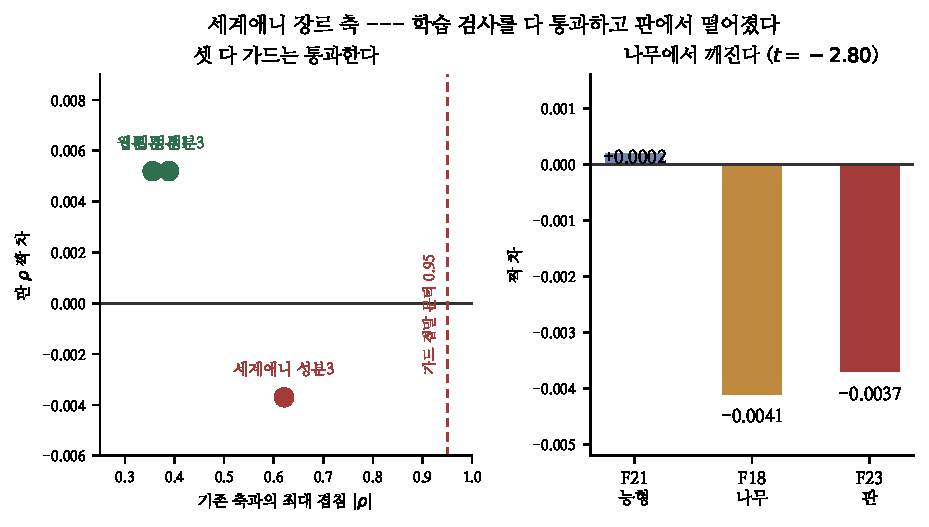
\includegraphics[width=\columnwidth]{figs/overlap.pdf}
\caption{왼쪽 --- 겹침과 판 이득. 셋 다 가드 문턱 왼쪽이다. 오른쪽 ---
세계애니 축이 어디서 깨지나.}
\end{figure}

\begin{center}\small
\begin{tabular}{lrrr}
\hline
 & 지금(19축) & $+$장르 & 짝 차 \\
\hline
F21 능형 & 0.4361 & 0.4363 & $+$0.0002 ($t{=}0.27$) \\
F18 나무 & 0.4532 & 0.4492 & $-$0.0041 ($t{=}-2.80$) \\
\textbf{F23 판} & \textbf{0.4623} & \textbf{0.4586} &
  $\mathbf{-0.0037}$ ($t{=}-3.02$) \\
\hline
세계애니 & 0.5203 & 0.5148 & $-$0.0054 ($t{=}-1.03$) \\
\hline
\end{tabular}
\end{center}

세계애니 자신은 잡음 안($t{=}-1.03$)인데 판이 뚜렷하게 내려간다. 그리고
\textbf{깨지는 곳이 나무다} --- 능형은 꿈쩍 안 한다.

\section{흐린 사본이었다}

겹침 0.621 의 상대를 봤다.

\begin{center}\small
\begin{tabular}{lr}
\hline
성분 3 이 겹치는 기존 축 & $\rho$ \\
\hline
\texttt{goods\_scale} & $+$0.621 \\
\texttt{target\_breadth} & $+$0.348 \\
\texttt{media\_push} & $+$0.313 \\
\hline
\end{tabular}
\end{center}

소스를 열었다.

\begin{quote}\small
\texttt{wanime\_axes.py:} \\
\texttt{\ a["goods\_scale"] = scale01(} \\
\texttt{\ \ \ log10(n\_episode * duration), 2.0, 4.0)}
\end{quote}

총 분량이다. 그리고 내 성분 3 은 \texttt{format} 토큰(TV · MOVIE · OVA ·
SPECIAL · TV\_SHORT)에 실려 있다. \textbf{포맷이 회차 수와 편당 길이를
정하므로 총 분량이 곧 포맷이다.} 극장판은 1회 $\times$ 120분, TV 는
12회 $\times$ 24분, OVA 는 그 사이 --- 같은 것을 두 번 말하고 있었다.

노트 240에서 태그 수가 \texttt{target\_breadth} 였던 것과 같은 사고이고,
이번엔 겹침이 1.000 이 아니라 0.621 이라 \textbf{가드가 안 잡았다.}

깨지는 곳이 나무인 것도 맞아떨어진다. 능형은 겹친 방향에 계수를 나눠 갖고
말지만, 나무는 \textbf{쪼갤 열이 하나 늘어} 같은 정보를 두 열로 나눠 자른다
--- 노트 242가 ``나무는 어긋나는 4\%를 문턱으로 쓴다''고 적은 것의 나쁜 쪽
얼굴이다. 그때는 겹친 열을 남겨 두는 것이 이득이었고 여기서는 손해다.
차이는 \textbf{새로 들어오는 정보가 있느냐}다.

\section{규약을 고친다}

\begin{center}\small
\begin{tabular}{lrr}
\hline
후보 & 최대 겹침 & 판 \\
\hline
웹툰 성분 1 & 0.356 & \multirow{2}{*}{$+$0.0052} \\
웹툰 성분 3 & 0.389 & \\
세계애니 성분 3 & \textbf{0.621} & $-$0.0037 \\
\hline
\end{tabular}
\end{center}

가드 \textbf{겹말}의 0.95 는 \emph{거부권} 문턱으로 정한 것이고(노트 240 ---
``막지 않고 이름표를 붙인다''), 그 자리에서는 옳다. 노트 242가 $\rho{=}1.000$
인 쌍도 못 빼는 경우를 보였으니 거부권 문턱은 높아야 한다.

\textbf{그런데 새 축을 채택할 때는 다른 문턱이 필요하다.} 채택은 ``새 정보가
있는가''를 묻는 것이고, 겹침 0.6 이면 정보의 대부분이 이미 있다. 점이 셋뿐이라
문턱 값을 정할 수는 없다(0.4 아래가 통과, 0.6 이 탈락). 값을 못 정하는 채로
\textbf{검사 항목에 넣는 것}까지가 이번에 정해진 것이다.

노트 239의 채택 검사가 이제 셋이다: 연도 통제 상관 · 시간 조각 부호 일치 ·
\textbf{기존 축과의 겹침}. 앞의 둘은 ``신호가 있는가''를 묻고 세 번째는
``그 신호가 새것인가''를 묻는다. \textbf{노트 240이 취소한 여섯 축도 앞의
둘은 다 통과했었다.}

\paragraph{남은 것}
\begin{center}\small
\begin{tabular}{ll}
\hline
갈래 & 왜 \\
\hline
겹침 문턱 & 점 셋으로는 못 정한다. 후보를 더 모으면 \\
세계애니 성분 4 & 겹침 0.212 인데 부호 4/5 로 떨어졌다 \\
게임 · 모바일 & 장르 문자열이 있나. 몫 8.6\% $+$ 16.9\% \\
만화 유보 6건 & 판에 못 닿는다. 수집이 필요한 유일한 자리 \\
\hline
\end{tabular}
\end{center}

\paragraph{규약} 새 축은 \textbf{학습 상관 · 조각 부호 · 겹침} 셋으로 본다.
앞의 둘만 보면 이미 있는 축의 흐린 사본이 통과한다 --- 그리고 흐린 사본은
나무를 깨뜨린다.

\end{document}
